\documentclass[aspectratio=169,11pt]{beamer}
\usetheme{Madrid}
\usecolortheme{default}
\usefonttheme{professionalfonts}

\usepackage[T1]{fontenc}
\usepackage[utf8]{inputenc}
\usepackage{lmodern}
\usepackage{amsmath,amssymb,mathtools}
\usepackage{booktabs}
\usepackage{tabularx}
\usepackage{graphicx}
\usepackage{array}
\usepackage{tikz}
\usetikzlibrary{arrows.meta,positioning,fit,calc,backgrounds}

\setbeamertemplate{navigation symbols}{}
\setbeamertemplate{footline}{\hfill\usebeamerfont{page number in head/foot}\insertframenumber\kern1em\vskip2pt}

\newcommand{\kk}{\Bbbk}
\newcommand{\R}{\mathbb{R}}
\newcommand{\Z}{\mathbb{Z}}
\newcommand{\Q}{\mathbb{Q}}
\newcommand{\TAMER}{\textsc{TAMER-OP}}
\newcommand{\multipers}{\textsc{multipers}}

\title{Implementation and ramifications of \TAMER: \\Toolkit for Algebraic Module Encodings over $\R^n$ and Other Posets}
\subtitle{Scope, flexibility, and efficiency in one system}
\author{Erik Mendes Novak\\
Mentor: Ezra Miller}
\date{April 9 2026}

\begin{document}

\begin{frame}
  
\includegraphics[width=1.6cm]{duke_logo.png}
  \titlepage
  
\centering
Thesis Defense
\end{frame}

\begin{frame}{What is a persistence module?}
\small
A persistence module is a functor
\[
M : Q \to \mathbf{Vect}_{\kk},
\]
where $Q$ is a poset and $\mathbf{Vect}_{\kk}$ is the category of vector spaces.

\medskip
\begin{itemize}
  \item Each parameter value $q \in Q$ carries a vector space $M(q)$.
  \item Each order relation $q \le q'$ carries a linear map
  \[
  M(q \le q') : M(q) \to M(q').
  \]
  \item Functoriality $\longleftrightarrow$ commutativity
\end{itemize}

\medskip
In ordinary persistence, $Q$ is a chain. In multiparameter persistence, $Q$ is often
\[
\Z^n \quad \text{or} \quad \R^n
\]
with the coordinatewise order.

\medskip
That is the source of both the expressive power and the computational difficulty.
\end{frame}

\begin{frame}{Why multiparameter persistence is hard}
\small
In one parameter, strong structure theorems lead to interval decompositions and barcodes.

\medskip
In several parameters, three problems appear immediately:
\begin{enumerate}
  \item the indexing poset is only partially ordered, not totally ordered;
  \item there is no barcode-style complete classification in general;
  \item analogs of intervals are infinitely or uncountably generated
\end{enumerate}

\medskip
So the practical question becomes:
\begin{quote}
How can we retain enough algebra to do meaningful computation, while still reducing the problem to finite data?
\end{quote}

\medskip
The answer in \TAMER{} is \emph{tameness} and \emph{finite encoding}.
\end{frame}

\begin{frame}{Tameness and finite encoding}
\small
A module is tame when it is constant on each of finitely many regions.

\medskip
\begin{block}{Finite encoding [Miller25]}
A module $M$ on a poset $Q$ is finitely encoded by
\begin{itemize}
  \item a finite poset $P$,
  \item a monotone classifier map $\pi : Q \to P$,
  \item and a $P$-module $H$,
\end{itemize}
such that the pullback satisfies
\[
M \cong \pi^* H.
\]
\end{block}

\medskip
A fringe presentation expresses a module in terms of indicator modules for upsets and downsets, via a finite matrix.

\medskip
This is the key computational move:
\begin{quote}
replace a large or infinite ambient parameter space by a finitely encoded module losslessly
\end{quote}
\end{frame}

\begin{frame}{The architecture: wide front end, thin center, wide output}
\small
\centering
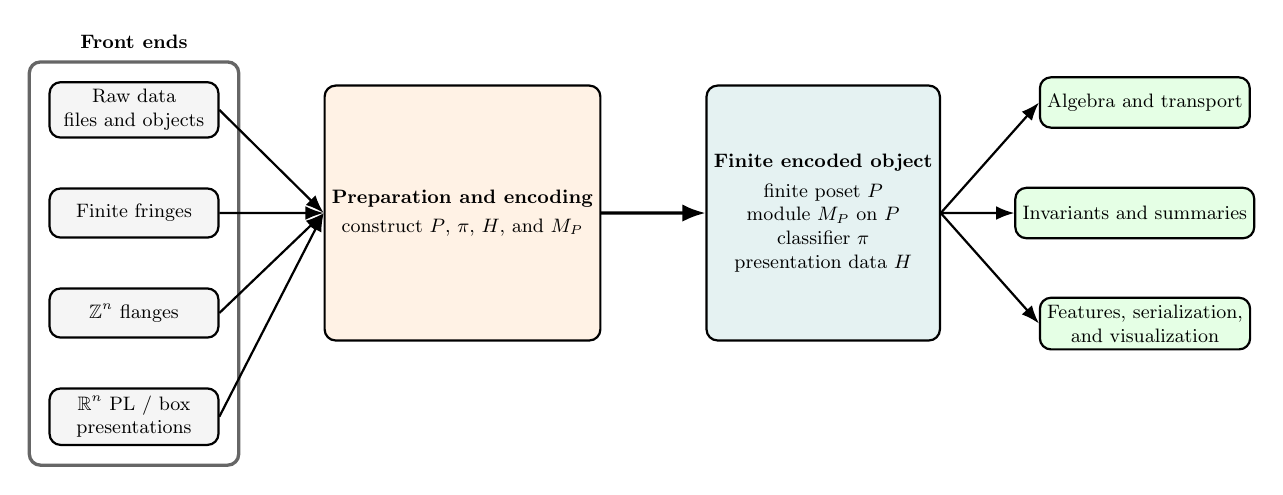
\begin{tikzpicture}[
    >=Latex,
    scale=0.78,
    transform shape,
    node distance=8mm and 10mm,
    every node/.style={font=\small},
    src/.style={rounded corners, draw, thick, align=center, minimum width=2.75cm, minimum height=0.8cm, fill=gray!8},
    stage/.style={rounded corners, draw, thick, align=center, minimum width=3.8cm, minimum height=1.0cm, fill=orange!10},
    outbox/.style={rounded corners, draw, thick, align=center, minimum width=3.0cm, minimum height=0.82cm, fill=green!10},
    layer/.style={rounded corners, draw=black!60, very thick, inner sep=7pt}
]

\node[src] (raw) {Raw data\\files and objects};
\node[src, below=of raw] (finite) {Finite fringes};
\node[src, below=of finite] (flange) {$\mathbb{Z}^n$ flanges};
\node[src, below=of flange] (pl) {$\mathbb{R}^n$ PL / box\\presentations};
\node[layer, fit=(raw)(finite)(flange)(pl), label={[yshift=0.2em]above:\textbf{Front ends}}] {};

\node[stage, right=17mm of finite, minimum height=4.15cm] (encode) {
\textbf{Preparation and encoding}\\[0.3em]
construct $P$, $\pi$, $H$, and $M_P$
};

\node[stage, right=17mm of encode, minimum height=4.15cm, fill=teal!10] (result) {
\textbf{Finite encoded object}\\[0.3em]
finite poset $P$\\
module $M_P$ on $P$\\
classifier $\pi$\\
presentation data $H$
};

\node[outbox, right=16mm of result, yshift=18mm] (alg) {Algebra and transport};
\node[outbox, right=12mm of result] (inv) {Invariants and summaries};
\node[outbox, right=16mm of result, yshift=-18mm] (feat) {Features, serialization,\\and visualization};

\draw[->, thick] (raw.east) -- (encode.west);
\draw[->, thick] (finite.east) -- (encode.west);
\draw[->, thick] (flange.east) -- (encode.west);
\draw[->, thick] (pl.east) -- (encode.west);
\draw[->, very thick] (encode.east) -- (result.west);
\draw[->, thick] (result.east) -- (alg.west);
\draw[->, thick] (result.east) -- (inv.west);
\draw[->, thick] (result.east) -- (feat.west);

\end{tikzpicture}

\medskip
\raggedright
This is the central claim of the software: heterogeneous inputs, one crucial encoding move, then many downstream options.
\end{frame}

\begin{frame}{Four input modes, one internal language}
\small
\centering
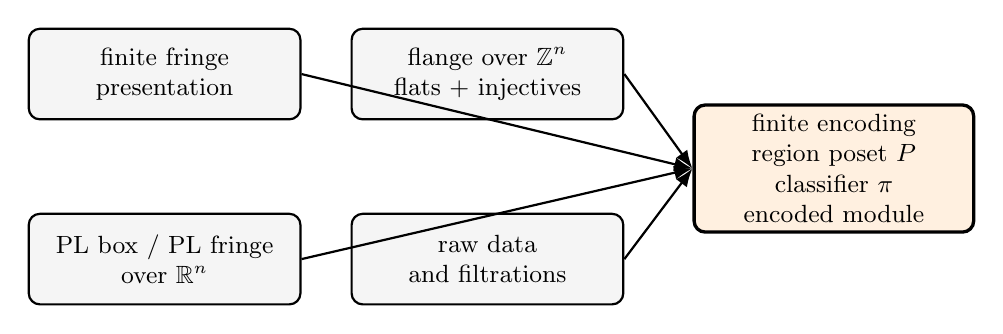
\begin{tikzpicture}[
  >=Latex,
  every node/.style={font=\small},
  src/.style={rounded corners, draw, thick, align=center, minimum width=3.45cm, minimum height=1.15cm, fill=gray!8},
  enc/.style={rounded corners, draw, very thick, align=center, minimum width=3.55cm, minimum height=1.2cm, fill=orange!12}
]
\node[src] (finite) at (-4.1,1.35) {finite fringe\\presentation};
\node[src] (flange) at (0,1.35) {flange over $\Z^n$\\flats + injectives};
\node[src] (pl) at (-4.1,-1.0) {PL box / PL fringe\\over $\R^n$};
\node[src] (raw) at (0,-1.0) {raw data\\and filtrations};
\node[enc] (enc) at (4.4,0.15) {finite encoding\\region poset $P$\\classifier $\pi$\\encoded module};
\draw[->,thick] (finite.east) -- (enc.west);
\draw[->,thick] (flange.east) -- (enc.west);
\draw[->,thick] (pl.east) -- (enc.west);
\draw[->,thick] (raw.east) -- (enc.west);
\end{tikzpicture}

\medskip
\raggedright
This is why \TAMER{} is flexible: the user can begin from the representation that is natural for the problem, but all roads lead to the same finite encoded object.
\end{frame}

\begin{frame}{Why encoding-first matters}
\small
\begin{columns}[T,totalwidth=\textwidth]
\column{0.32\textwidth}
\begin{block}{Scope}
One system for:
\begin{itemize}
  \item raw data ingestion,
  \item $\Z^n$ and $\R^n$ front ends,
  \item finite encodings,
  \item exact algebra,
  \item invariants, geometry, and export.
\end{itemize}
\end{block}

\column{0.32\textwidth}
\begin{block}{Flexibility}
Users do not have to commit to a single invariant too early.

\medskip
The encoded module can be inspected algebraically before choosing rank, slice, image, or geometric summaries.
\end{block}

\column{0.32\textwidth}
\begin{block}{Efficiency}
Encoding removes redundant ambient information while keeping what later computation needs.

\medskip
That gives both tractability and speed.
\end{block}
\end{columns}
\end{frame}

\begin{frame}{Project scope at a glance}
\small
\begin{columns}[T,totalwidth=\textwidth]
\column{0.55\textwidth}
\begin{itemize}
  \item \textbf{65000 lines of code} in just the source files
  \item \textbf{37 source files} in the present codebase snapshot.
  \item \textbf{4 front end input modes}: finite fringe, flange, PL box / PL fringe, and raw data.
  \item \textbf{130+ named invariant, distance, geometry, and support routines} in the current invariant layer.
  \item \textbf{100+ named algebraic and homological constructions} across exact-category, resolution, complex, and derived-functor layers.
  \item Support for \textbf{$\mathbb{Z}^n$, $\mathbb{R}^n$, and finite posets} inside the same workflow.
\end{itemize}

\column{0.4\textwidth}
\begin{block}{Why this matters}
This is not a narrow experimental codebase built around one descriptor.

\medskip
It is a broad computational environment for encoded multiparameter persistence.
\end{block}
\end{columns}
\vfill
{\tiny Counts are taken from the project snapshot on 9 April 2026 and the exported invariant/algebra layers used in the thesis and companion decks.}
\end{frame}

\begin{frame}{What users can do after encoding: invariants}
\small
\renewcommand{\arraystretch}{1.15}
\begin{tabular}{p{0.29\textwidth} p{0.39\textwidth} p{0.24\textwidth}}
\toprule
Family & Examples & Output object \\
\midrule
Rank and dimension & restricted Hilbert, rank invariant, rectangle signed measures & vectors, rank tables, sparse signed data \\
Slice-based & slice barcodes, matching distance, sliced bottleneck / Wasserstein & barcodes, scalar distances \\
Function/image summaries & multiparameter landscape, MPPI & tensors, raster images \\
Euler and signed measures & Euler surface, Euler signed measure, point signed measure & grids, sparse signed point measures \\
Geometry-aware summaries & support measure, aspect ratio, interface measure, module geometry summary & scalars, histograms, weighted summaries \\
Support-theoretic & Betti/Bass support, socle, associated primes & finite algebraic descriptors \\
\bottomrule
\end{tabular}

\medskip
\raggedright
The key message: no single invariant is enough, so the software implements a family of invariant types specialized to different needs.
\end{frame}

\begin{frame}{What users can do after encoding: algebra}
\small
\begin{columns}[T,totalwidth=\textwidth]
\column{0.52\textwidth}
\textbf{Exact-category layer}
\begin{itemize}
  \item kernels, images, cokernels, quotients
  \item submodules and inclusions
  \item pullbacks, pushouts, equalizers, coequalizers
  \item short exact sequences and snake lemma
\end{itemize}

\textbf{Resolution and derived layer}
\begin{itemize}
  \item projective covers and injective hulls
  \item indicator resolutions
  \item Hom, Ext, Tor
  \item long exact sequences
\end{itemize}

\column{0.45\textwidth}
\textbf{Complex-level layer over encoding poset $P$}%
\begin{itemize}
  \item mapping cones and distinguished triangles
  \item RHom and derived tensor
  \item hyperExt and hyperTor
  \item spectral-sequence infrastructure
\end{itemize}

\medskip
\begin{block}{Why this is unusual}
Most multiparameter workflows stop after constructing an invariant.

\medskip
\TAMER{} keeps the module itself, so users can do algebra \emph{before} they summarize.
\end{block}
\end{columns}
\end{frame}

\begin{frame}{Representative benchmark: full pipeline speedups over \multipers}
\small
\centering
\begin{tabular}{lcccccc}
\toprule
Invariant & Rips & Codensity rips & Rips lowerstar & Landmark & Alpha & Cubical \\
\midrule
Euler & 5.4 & 7.5 & 13.7 & 5.6 & 26.4 & 26.8 \\
rank signed measure & $\infty$ & $\infty$ & $\infty$ & $\infty$ & $\infty$ & $\infty$ \\
slice barcodes & 3.7 & 3.2 & 3.5 & 5.1 & -- & 9.5 \\
mp\_landscape & 4.8 & 2.7 & 5.5 & 6.0 & -- & 11.2 \\
restricted\_hilbert & -- & 1.33 & 1.24 & -- & 25.2 & -- \\
rank\_invariant & $\infty$ & $\infty$ & $\infty$ & $\infty$ & $\infty$ & $\infty$ \\
\bottomrule
\end{tabular}

\medskip
\raggedright
Numbers are speedup factors for \TAMER{} over \multipers{} on the supplied end-to-end ingestion-plus-invariant benchmarks.

\medskip
\begin{itemize}
  \item ``$\infty$'' means no tractable \multipers{} result on that benchmark.
  \item The important point is not just that \TAMER{} is faster on overlapping tasks, but that it also supports broader encoded workflows.
\end{itemize}
\end{frame}

\begin{frame}{Why these benchmarks matter}
\small
\begin{columns}[T,totalwidth=\textwidth]
\column{0.5\textwidth}
\begin{block}{Near-term message}
Even on the tasks that other tools already attempt, the encoding-first approach is highly competitive and often much faster.
\end{block}

\column{0.46\textwidth}
\begin{block}{Long-term message}
The point is not merely speed. Encoding creates a finite middle ground:
\begin{itemize}
  \item enough compression to be tractable,
  \item enough structure to keep exact algebra alive.
\end{itemize}
\end{block}
\end{columns}

\vspace{0.5em}
\centering
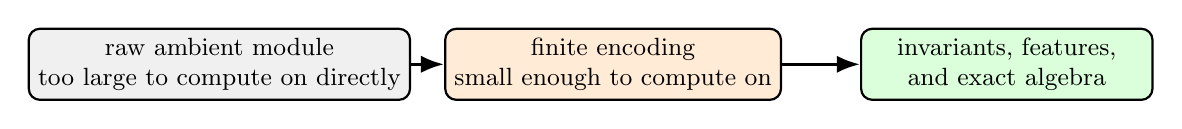
\begin{tikzpicture}[
  >=Latex,
  every node/.style={font=\small},
  box/.style={rounded corners, draw, thick, align=center, minimum width=3.7cm, minimum height=0.9cm}
]
\node[box, fill=gray!12] (raw) at (0,0) {raw ambient module\\too large to compute on directly};
\node[box, fill=orange!16] (enc) at (5.0,0) {finite encoding\\small enough to compute on};
\node[box, fill=green!14] (sum) at (10.0,0) {invariants, features,\\and exact algebra};
\draw[->, very thick] (raw) -- (enc);
\draw[->, very thick] (enc) -- (sum);
\end{tikzpicture}
\end{frame}

\begin{frame}{Visualization examples: Rips codensity bifiltration snapshot}
	\centering
    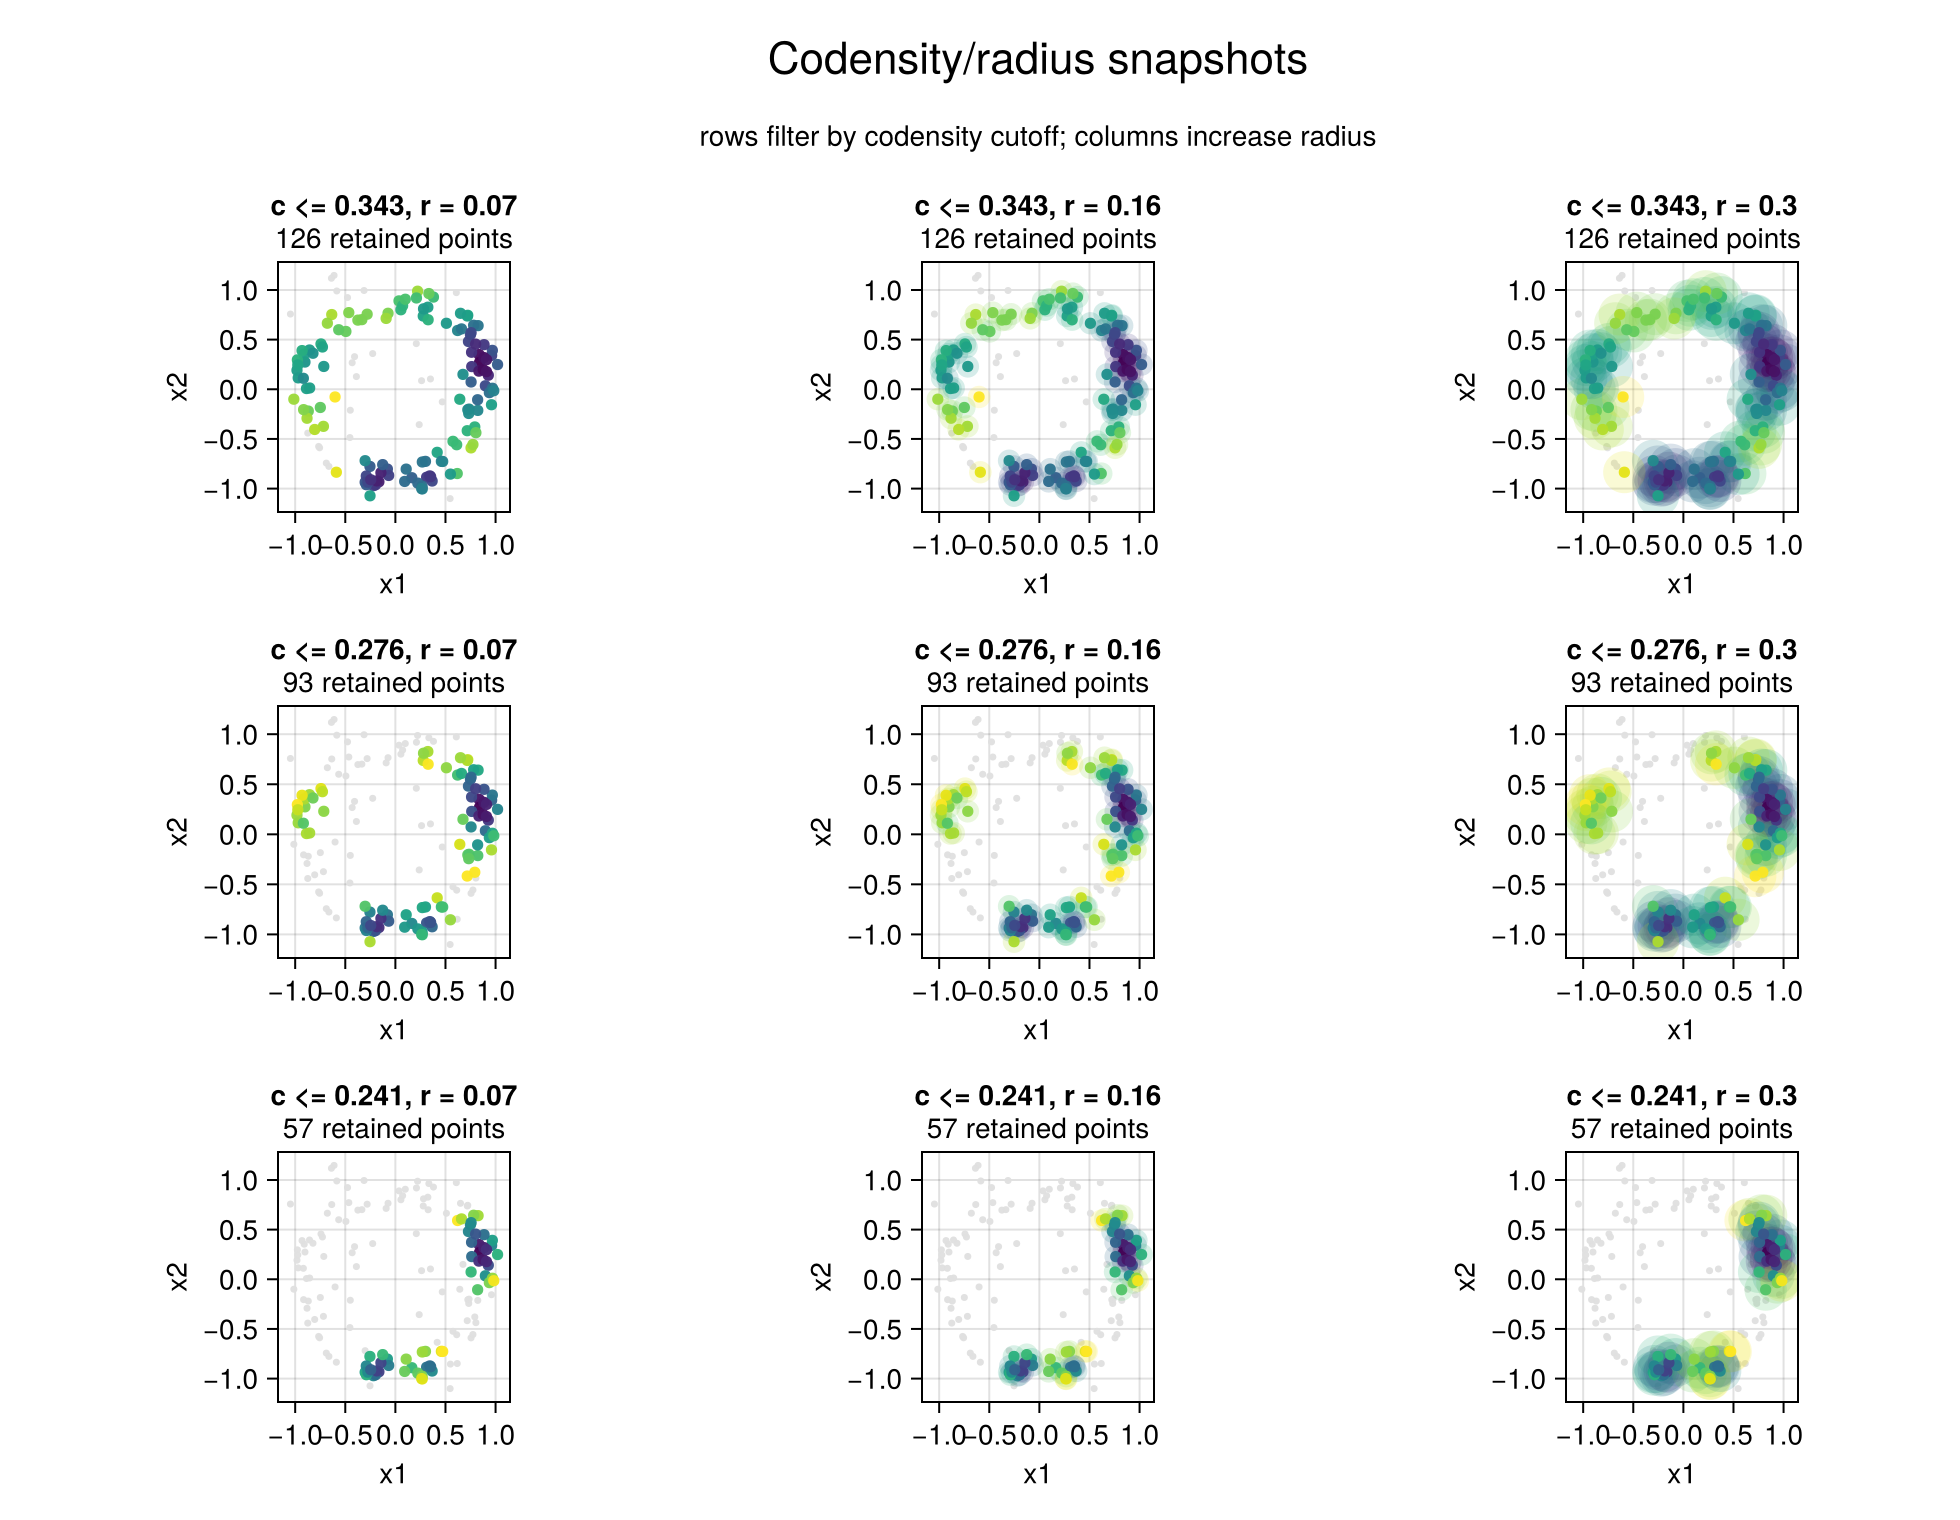
\includegraphics[width=10cm]{annulus_codensity_radius_snapshots.png}

\end{frame}

\begin{frame}{Visualization examples: Annulus $H_1$ support plane for Rips codensity}
	\centering
	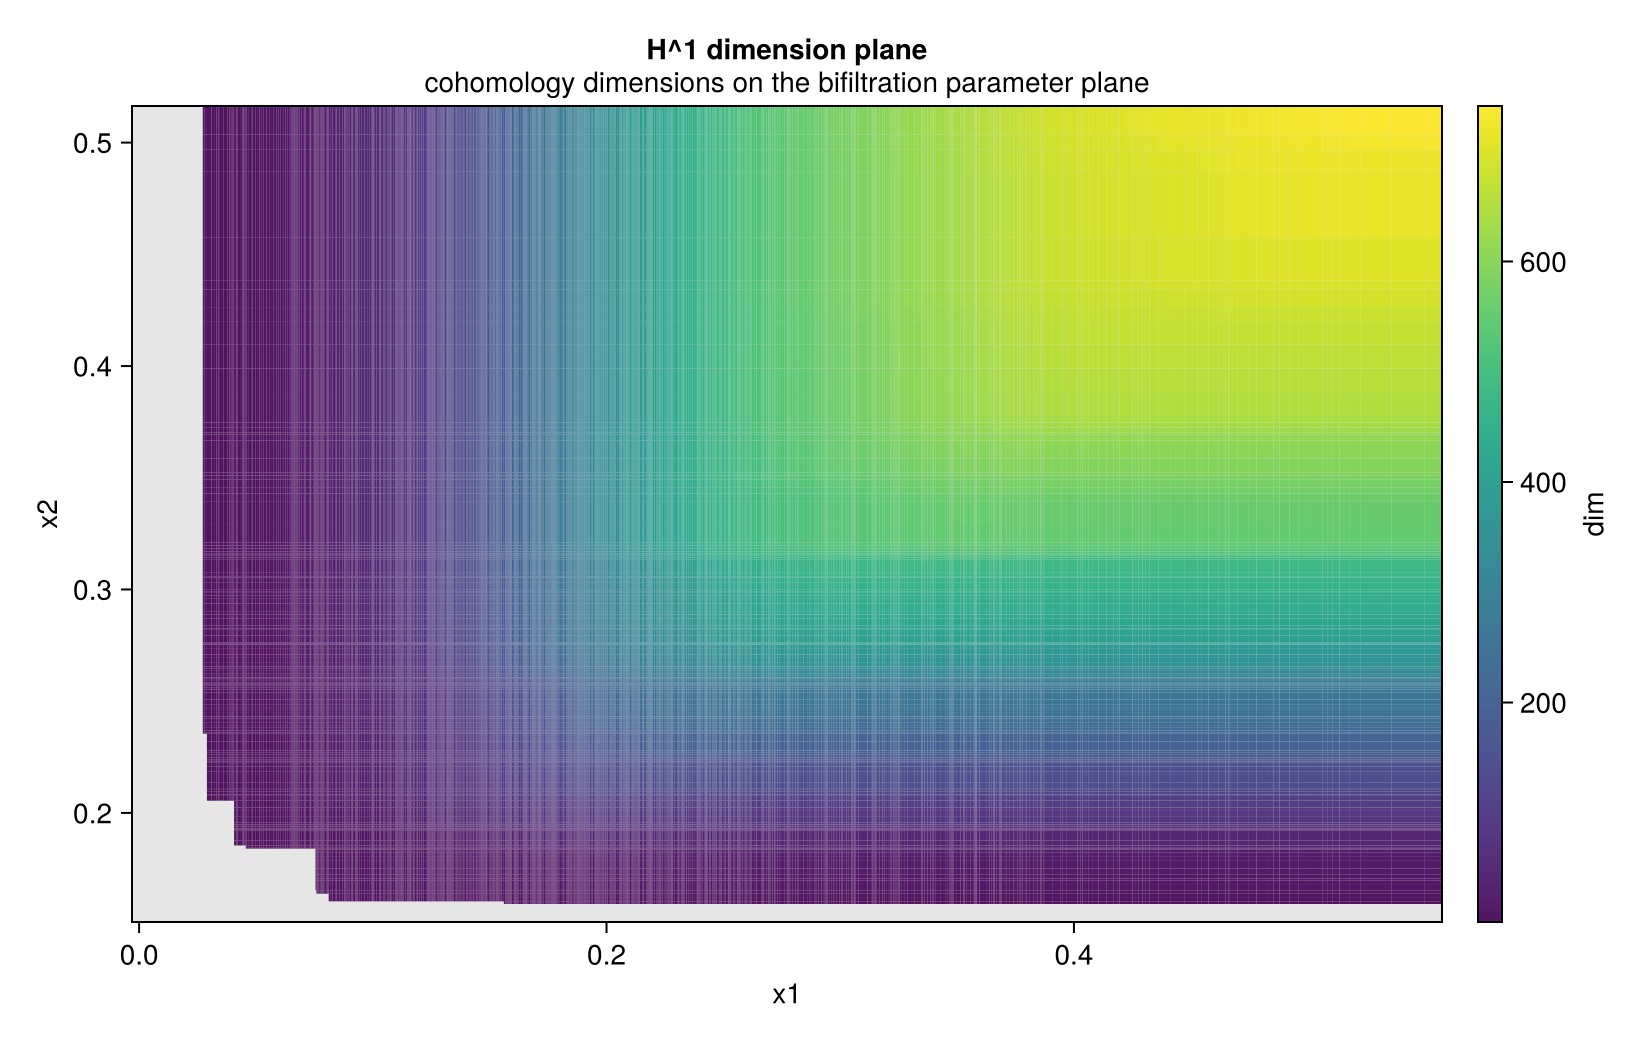
\includegraphics[width=10cm]{annulus_h1_support_plane.png}
	
\end{frame}

\begin{frame}{Visualization examples: Rank heatmap}
	\centering
	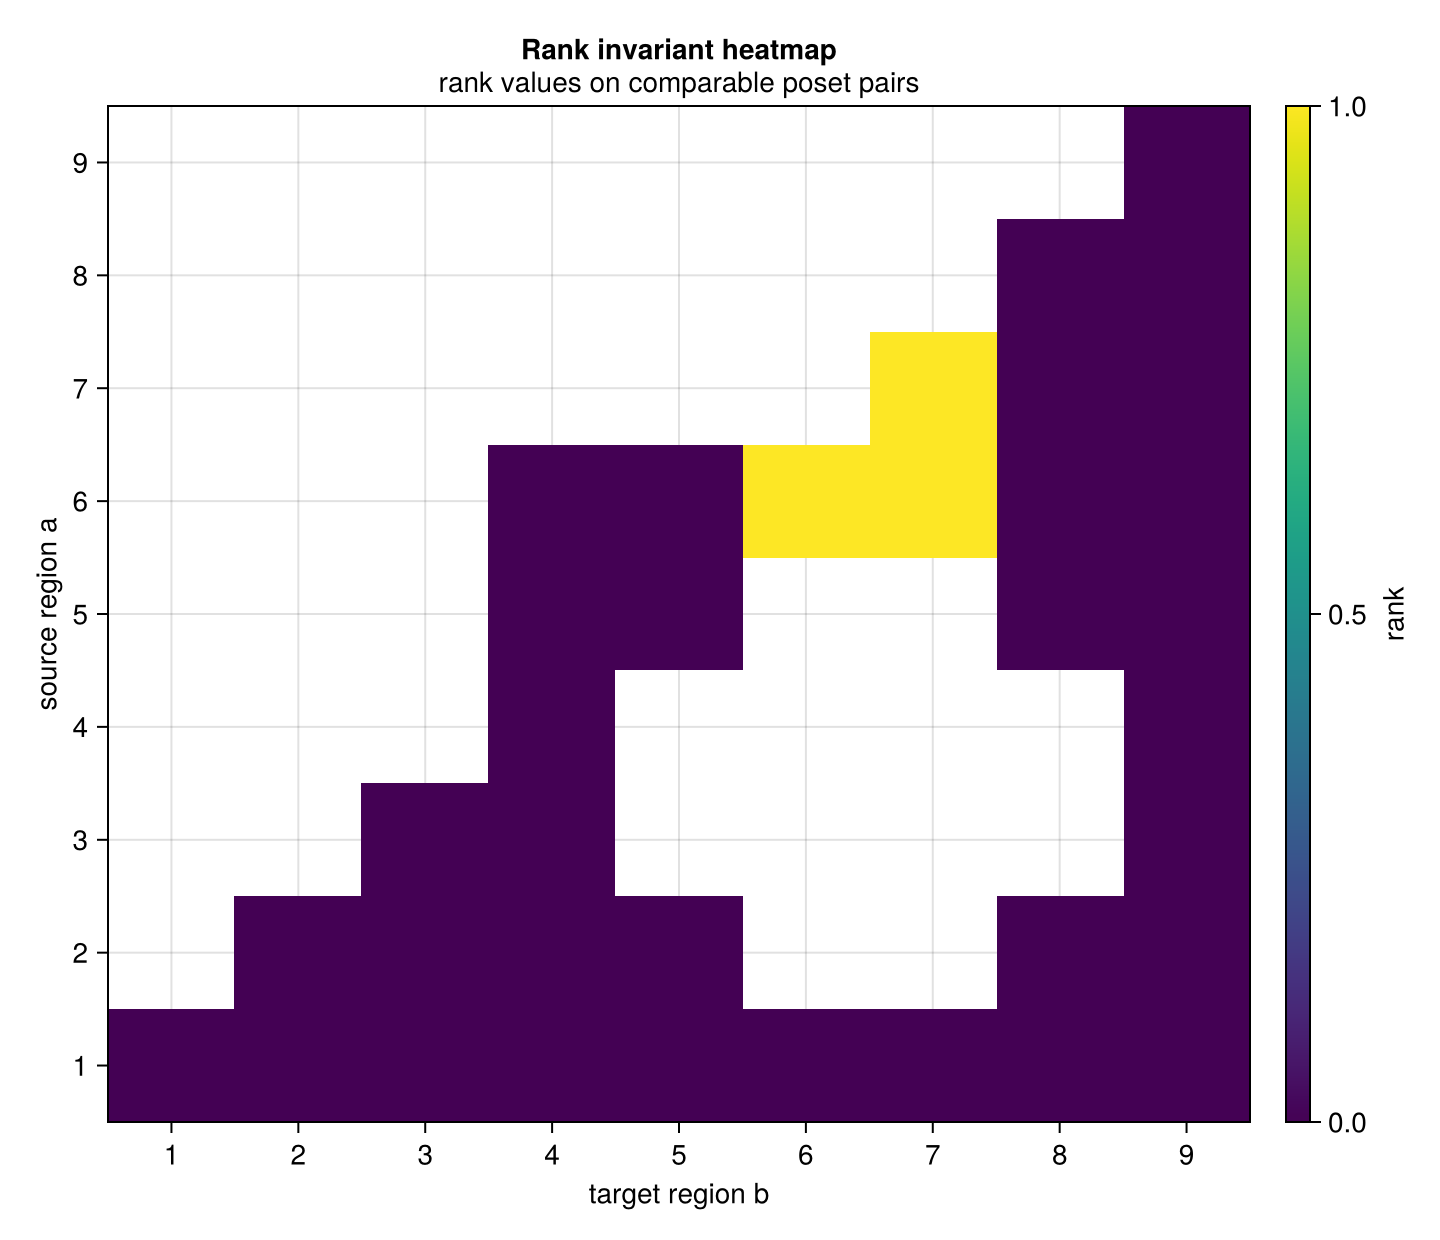
\includegraphics[width=8cm]{rank_heatmap.png}
	
\end{frame}

\begin{frame}{Visualization examples: Visual of an MPP image}
	\centering
	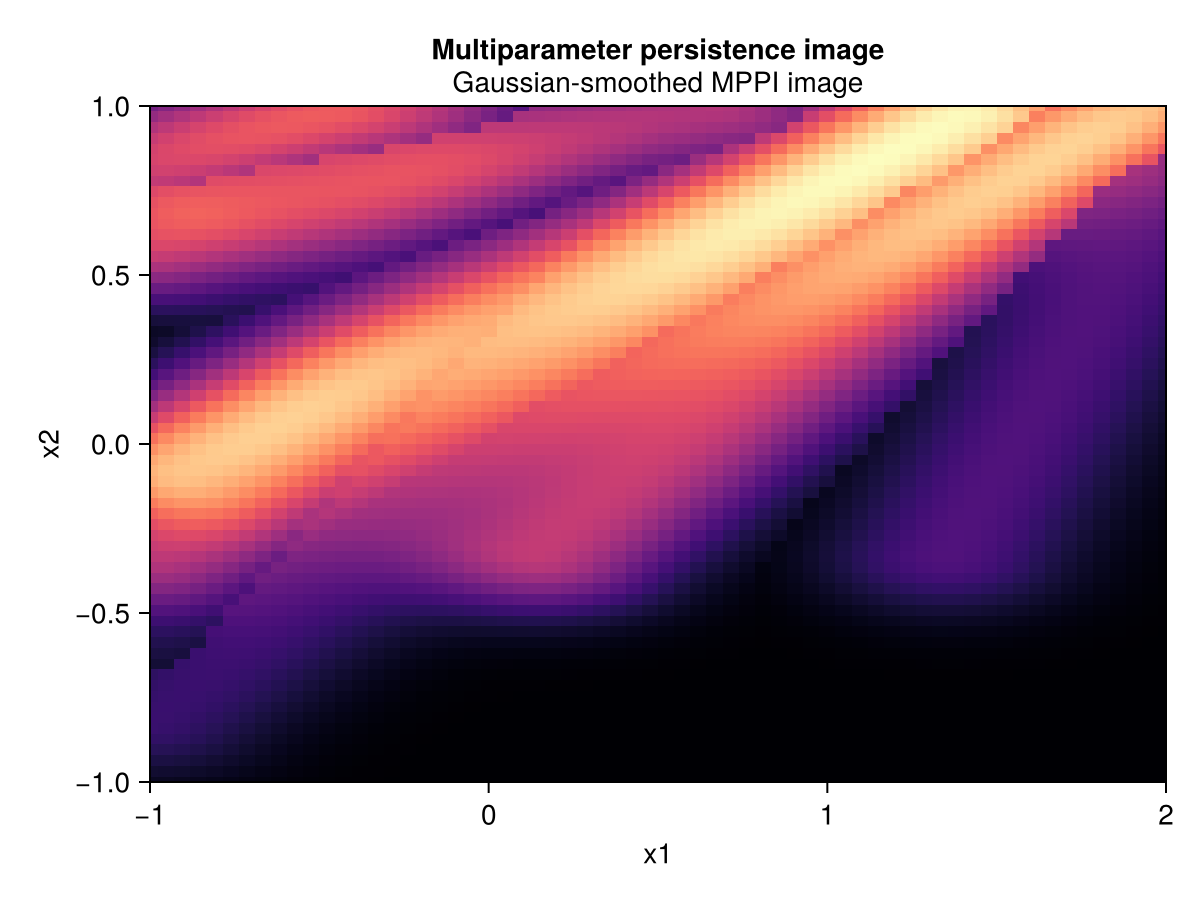
\includegraphics[width=10cm]{visual_mpp_image.png}
	
\end{frame}

\begin{frame}{Visualization examples: Encoding of a PL box}
	\centering
	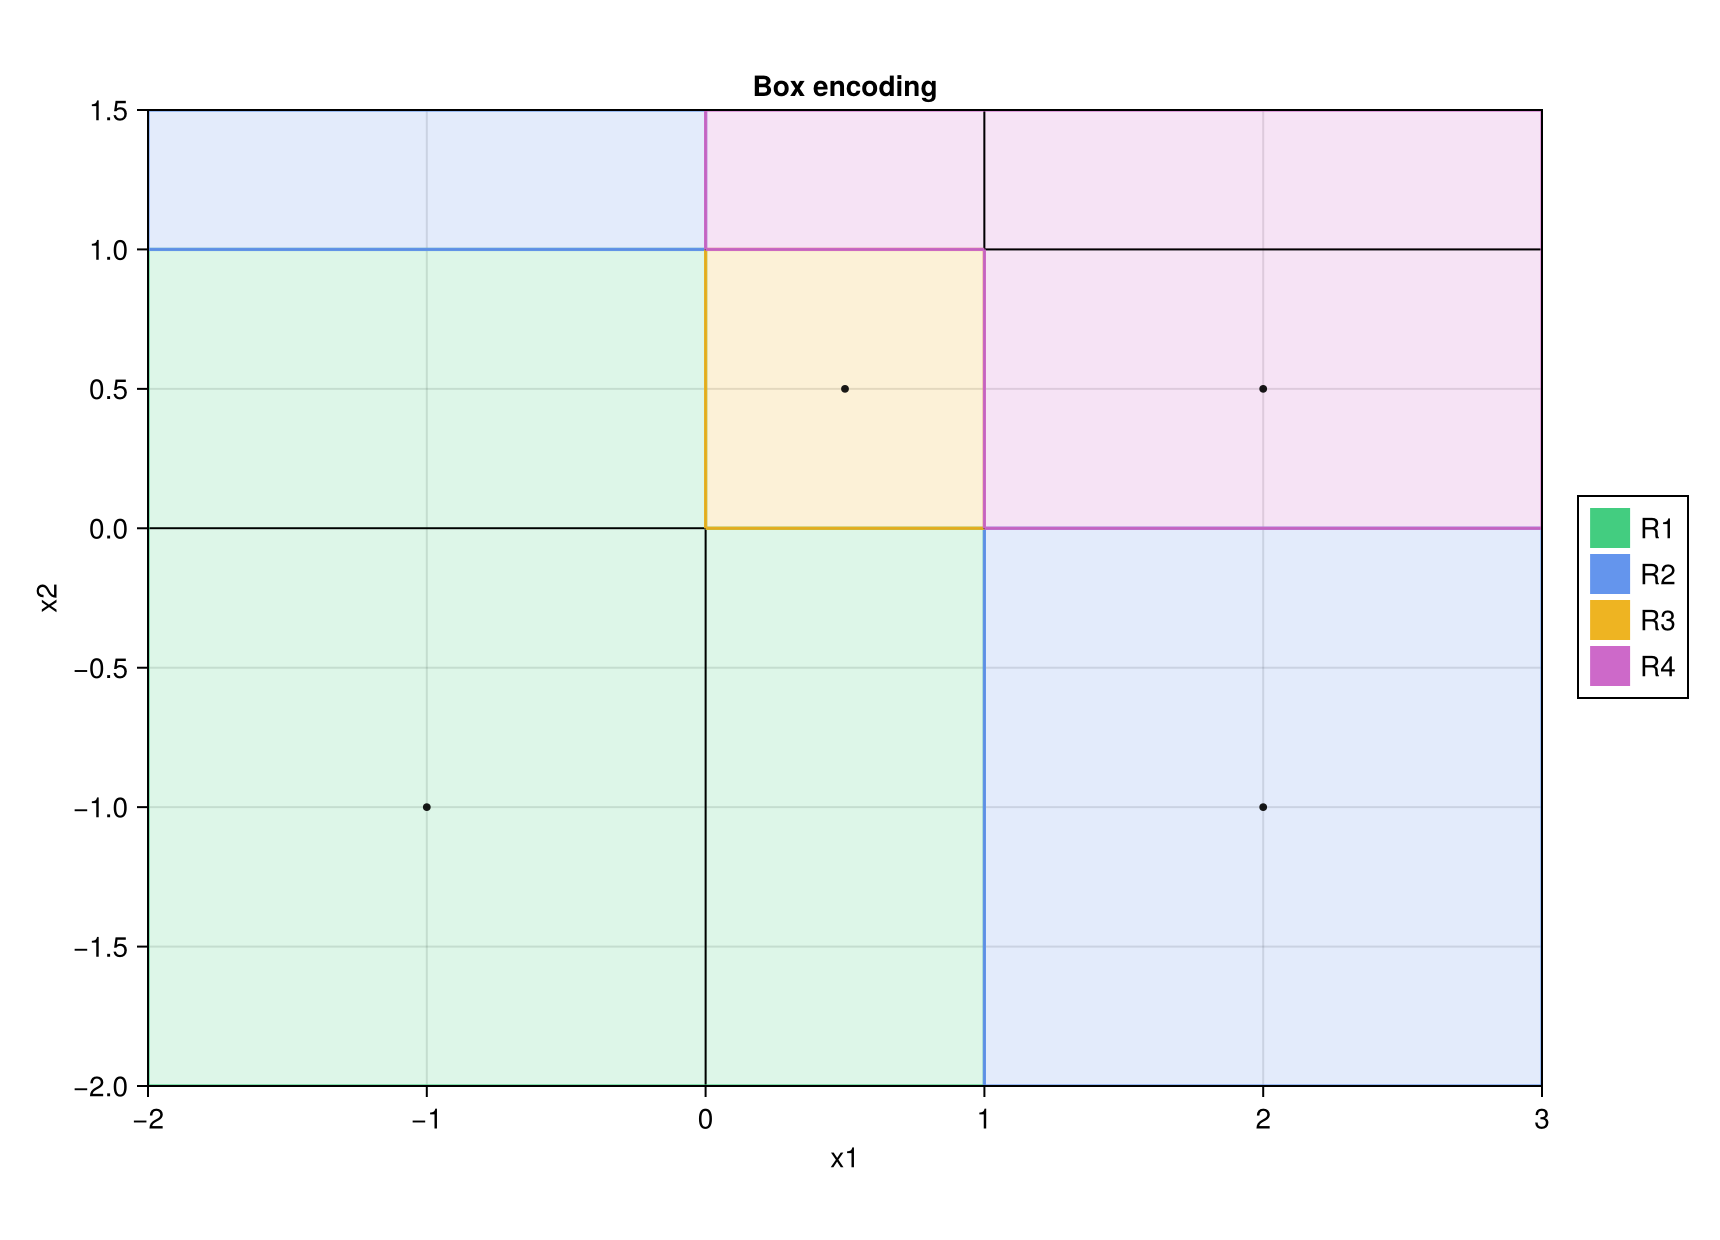
\includegraphics[width=10cm]{kernel_smoke_regions.png}
	
\end{frame}


\begin{frame}{What need does \TAMER{} fill?}
\small
\begin{itemize}
  \item It treats finite encoding as the central computational move, not as an afterthought.
  \item It supports raw data, $\Z^n$ presentations, $\R^n$ presentations, and finite-poset modules in one framework.
  \item It keeps the module available for exact algebra, rather than forcing an invariant too early.
  \item It supports broad invariant families and geometry-aware summaries after encoding.
  \item On overlapping pipeline tasks, it is already highly competitive and often substantially faster than current alternatives.
\end{itemize}

\medskip
\begin{block}{Takeaway}
If multiparameter persistence is going to become a practical algebraic technology rather than a collection of isolated summaries, then we need an encoding-first system. That is the niche \TAMER{} is built to fill.
\end{block}
\end{frame}

\begin{frame}{Deployment and use}
	The software is already finding use in projects and natural interest in the community:
	\begin{itemize}
		\item Ramachandran plots and protein folding work with Dr. Michael Prisant and Dr. Jane Richardson at Duke
		\item Implementation discussions with Jan Jendrysiak of TU Munich, soon in Oxford
		\item I will road show it at SoCG 2026
		\item The repo already has 14 stars on Github
		\item 1-hour tutorial at Combinatorial Coworkspace in Kleinwalsertal, Austria, in March 2026
		\item Soon: interaction with David Loiseaux, creator of MULTIPERS
	\end{itemize}
\end{frame}

\begin{frame}{AI disclaimer}
	AI was used strictly for:
	\begin{itemize}
		\item Writing docstring for the code
		\item Guiding research direction, especially in invariants
		\item Creating TikZ diagrams
		\item Helping generate tests
		\item Writing boilerplate for benchmark harnesses
		\item Diagnosing Julia inefficiencies
		\item Writing the linear algebra backend
		\item Making the API user-friendly
	\end{itemize}
    
    All use of AI was strictly monitored and cross-checked.
	
\end{frame}

\begin{frame}{Github}
	\centering
	\Large{\textbf{www.github.com/erikmnovak/TamerOp.jl}}
\end{frame}


% =========================================================
% Bibliography Slides
% =========================================================

\begin{frame}{References}
	\tiny
	\begin{thebibliography}{99}
		
		\bibitem{Mil20}
		E.~Miller.
		\newblock \emph{Homological algebra of modules over posets}.
		\newblock arXiv:2008.00063, 2020.
		
		\bibitem{Waa24}
		L.~Waas.
		\newblock \emph{Notes on abelianity of categories of finitely encodable persistence modules}.
		\newblock arXiv:2407.08666, 2024.
		
		\bibitem{Mil23}
		E.~Miller.
		\newblock \emph{Stratifications of real vector spaces from constructible sheaves}.
		\newblock J. Appl. Comput. Topol., 2023.
		
		\bibitem{KS18}
		M.~Kashiwara and P.~Schapira.
		\newblock \emph{Persistent homology and microlocal sheaf theory}.
		\newblock JACT, 2018.
		
		\bibitem{CB15}
		W.~Crawley-Boevey.
		\newblock \emph{Decomposition of pointwise finite-dimensional persistence modules}.
		\newblock J. Algebra Appl., 2015.
		
		\bibitem{ZC05}
		A.~Zomorodian and G.~Carlsson.
		\newblock \emph{Computing persistent homology}.
		\newblock DCG, 2005.
		
	\end{thebibliography}
\end{frame}

\begin{frame}{References (continued)}
	\tiny
	\begin{thebibliography}{99}
		
		\bibitem{CZ09}
		G.~Carlsson and A.~Zomorodian.
		\newblock \emph{The theory of multidimensional persistence}.
		\newblock DCG, 2009.
		
		\bibitem{CEH07}
		D.~Cohen-Steiner, H.~Edelsbrunner, and J.~Harer.
		\newblock \emph{Stability of persistence diagrams}.
		\newblock DCG, 2007.
		
		\bibitem{ELZ02}
		H.~Edelsbrunner, D.~Letscher, and A.~Zomorodian.
		\newblock \emph{Topological persistence and simplification}.
		\newblock DCG, 2002.
		
		\bibitem{Les15}
		M.~Lesnick.
		\newblock \emph{The interleaving distance on multidimensional persistence modules}.
		\newblock FoCM, 2015.
		
		\bibitem{LW15}
		M.~Lesnick and M.~Wright.
		\newblock \emph{Interactive visualization of 2-D persistence modules}.
		\newblock arXiv:1512.00180.
		
		\bibitem{CDSGO16}
		F.~Chazal et al.
		\newblock \emph{The Structure and Stability of Persistence Modules}.
		\newblock Springer, 2016.
		
	\end{thebibliography}
\end{frame}

\begin{frame}{References (continued)}
	\tiny
	\begin{thebibliography}{99}
		
		\bibitem{Oud15}
		S.~Oudot.
		\newblock \emph{Persistence Theory}.
		\newblock AMS, 2015.
		
		\bibitem{EH10}
		H.~Edelsbrunner and J.~Harer.
		\newblock \emph{Computational Topology}.
		\newblock AMS, 2010.
		
		\bibitem{Mac98}
		S.~Mac Lane.
		\newblock \emph{Categories for the Working Mathematician}.
		\newblock Springer, 1998.
		
		\bibitem{Wei94}
		C.~Weibel.
		\newblock \emph{An Introduction to Homological Algebra}.
		\newblock Cambridge, 1994.
		
		\bibitem{Eis95}
		D.~Eisenbud.
		\newblock \emph{Commutative Algebra}.
		\newblock Springer, 1995.
		
		\bibitem{MS05}
		E.~Miller and B.~Sturmfels.
		\newblock \emph{Combinatorial Commutative Algebra}.
		\newblock Springer, 2005.
		
	\end{thebibliography}
\end{frame}

\end{document}
